% \chapter{Systém trasování v ČR od října 2020 do května 2021: jeho výkon, reporting a (ne)využívání dat pro jeho řízení}\label{Trasovani}
\chapter[Systém trasování v~ČR]{Systém trasování v~ČR: efektivita, reporting a~(ne)využívání dat}\label{Trasovani}

\textit{Jakub Drbohlav, Eva Blechová}
\vspace{15mm}

\section*{Úvod}

Identifikace rizikových kontaktů (tzv. trasování, z~anglického „tracing“) je jednou z~klíčových metod, jak udržet jakoukoli epidemii infekční nemoci pod kontrolou nebo přinejmenším jak snížit její reprodukční číslo. Cílem trasování je přerušit šíření epidemie identifikací všech osob, které byly v~kontaktu s~nakaženým, jejich testováním a izolací (test, trace, isolate).

Podobné metody se začaly využívat v~Anglii již od poloviny 19. století \cite{pg:mooney2020} V~případě covid-19 vedou i jednoduché trasovací strategie k~výraznému snížení reprodukčního čísla: pouhá izolace osob sdílejících domácnost o~29 \%, trasování všech rizikových kontaktů pozitivního případu až o~64 \% \cite{pg:kucharski2020}.

Podobně jako další státy bývalého komunistického bloku měla ČR na počátku pandemie covid-19 rozvinutou síť hygienické služby s~dlouhou tradicí působení. Odpovědnost za trasování od počátku pandemie připadala na krajské hygienické stanice (KHS) pod vedením hlavní hygieničky (která je zároveň náměstkyní ministra zdravotnictví). Do této role byla v~březnu 2020 jmenována Jarmila Rážová, po roce ji ve funkci v~březnu 2021 nahradila Pavla Svrčinová.

KHS od počátku pandemie fungovaly velmi autonomně, s~vlastními postupy, způsoby práce a bez jednotného IT řešení. Klíčovým posunem jejich práce bylo zavedení jednotného IT systému pro trasování od společnosti Daktela\footnote{\url{https://www.daktela.com/trasovaci-callcentrum/}}. Zavádění systému začalo v~dubnu 2020 a bylo plně implementováno v~praxi všech pracovníků a pracovnic KHS v~září 2020.

Díky jednotnému IT systému je výrazně usnadněno nejen sdílení kapacit mezi jednotlivými KHS (které bylo do té doby nemožné), ale také zapojení externích posil (nejdříve AČR, PČR, Celní a finanční správy, jakožto i firem na dobrovolnické bázi, od prosince 2020 profesionálních call center). Postupně také docházelo k~lepšímu propojení systému s~IT systémy státu (ISIN, systém eŽádanky) a k~obohacení systému o~nové prvky (sebetrasování pozitivních a od května 2021 i rizikových kontaktů).

Díky jednotnému IT systému bylo zároveň možné sledovat výkon systému trasování v~ČR a v~ideálním případě jej i pravidelně hodnotit a řídit. Ministerstvo zdravotnictví, respektive tým Chytré karantény ve spolupráci s~dodavatelem IT systému Daktela začal od října 2020 denně zveřejňovat detailní reporting výkonu českého systému trasování.

Od listopadu 2020 jsme na webových stránkách BISOP publikovali pravidelný monitoring trasování, k~dnešnímu datu dospěl k~devíti vydáním. Jeho součástí byla vždy analýza výsledků trasování, stejně jako doporučení ke zlepšení \cite{tr_bisop07}. 

Cílem tohoto textu je zhodnotit systém trasování v~ČR. Zaměřujeme se na období osmi měsíců (od října 2020 do května 2021), protože pro období březen--září 2020 neexistují dostatečně kvalitní data. V~první části textu si klademe otázku, zda systém reportování (zejména vybrané indikátory) a jeho využití byly přizpůsobeny pandemické situaci. V~druhé části pak analyzujeme vývoj výkonu trasování na základě dvou hlavních indikátorů -- rychlosti trasování a počtu rizikových kontaktů.

\section*{Metody}

Naším hlavním zdrojem jsou data reportingu trasování. Tým Chytré karantény (respektive dodavatel IT systému Daktela) začal publikovat pravidelná denní data o~kvalitě trasování na webu mimisterstva zdravotnictví ČR počínaje 13. říjnem 2020 (viz report z~13. října na obr. \ref{fig:daktela} níže). Report obsahuje mnoho detailních údajů pro celou ČR a pro jednotlivé kraje.

Pro zahraniční srovnání využíváme obdobná veřejně dostupná data reportingu trasování s~uvedením zdroje.

Kromě primárních dat využíváme rešerše zahraniční praxe a rešerše veřejných vyjádření osob odpovědných za systém trasování v~ČR, veřejných dokumentů vlády a zveřejněného dokumentu doporučení pro prevenci druhé vlny covid-19 z~27. května 2020.

Dále se budeme věnovat:
\begin{itemize}
\item zvoleným indikátorům reportingu trasování v~ČR, jejich vhodnosti, srovnání se zahraničními systémy a tomu, jak byje  bylo možné náležitě doplnit,
\item systému řízení trasování a jeho nedostatkům,
\item výkonu trasování s~ohledem na dva klíčové indikátory jeho výstupů, rychlost a počet identifikovaných rizikových kontaktů.
\end{itemize}

% \subsection*{Systém reportování, indikátory a způsob jeho využívání}

\paragraph{Systém reportování, indikátory a způsob jeho využívání.} V~tomto oddíle se budeme zabývat především zvoleným indikátorům reportingu trasování a tomu, jak byly využívány v~systému řízení trasování.

Hlavní indikátory reportingu se zaprvé zaměřují na vstupy:
\begin{itemize}
\item počet operátorů (trasovačů) denně,
\item počet hovorů pozitivním případům a jejich rizikovým kontaktům.
\end{itemize}

Zadruhé sledují výstupy trasování:
\begin{itemize}
\item podíl vytrasovaných pozitivních případů do 24 h,
\item podíl vytrasovaných rizikových kontaktů do 24 h,
\item počet identifikovaných rizikových kontaktů na jeden případ,
\item počet nevyřešených hovorů.
\end{itemize}

\begin{figure}[ht]
    \centering
    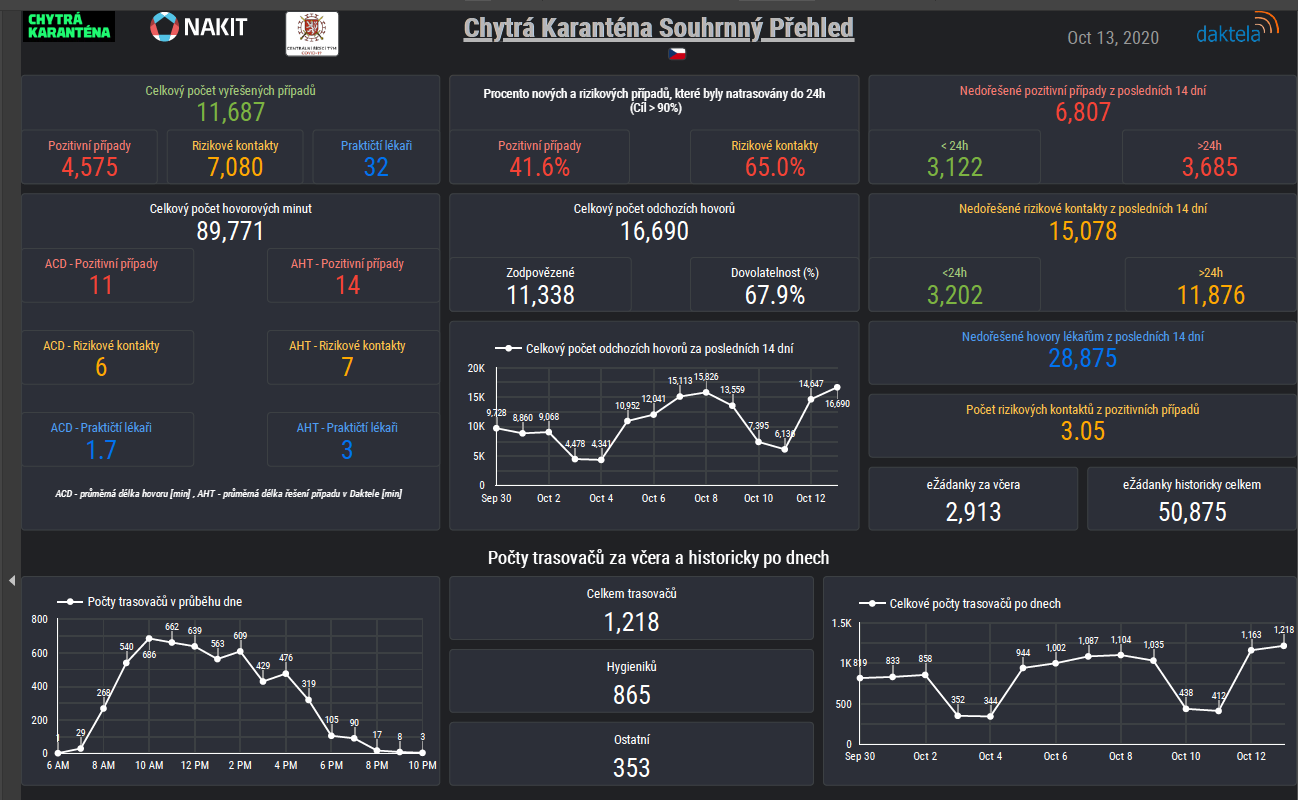
\includegraphics[width=0.8\textwidth]{./pic/daktela.jpg}
    \caption{Denní report z~13. října 2020.}
    \label{fig:daktela}
\end{figure}



Z~pohledu zahrnutých indikátorů je využívaná sada nastavená dostatečně pře\-de\-vším pro řízení kapacit trasování (důraz na objem a proces) a pro základní informace o~kvalitě trasování (podíl případů vytrasovaných do 24 h a počet identifikovaných rizikových kontaktů).

Tyto indikátory jsou standardně využívané i v~dalších zemích (Francie, Velká Británie, země jihovýchodní Asie), doporučuje je WHO \cite{tr_WHO_2021}, European Centre for Disease Prevention and Control \cite{tr_ECDC_2020}, americké Center for Disease Control and Prevention \cite{tr_CDC_2020} nebo nadace Resolve to save lives \cite{tr_contact_tracing}.

Rozšíření reportingu trasování jsme pravidelně navrhovali v~našem monitoringu trasování od jeho prvního vydání v~listopadu 2020 \cite{tr_bisop07}.

Reporting trasování v~ČR totiž nezahrnuje sofistikovanější indikátory zaměřené na jeho kvalitu či celkovou dostatečnost systému. Z~kombinace rychlosti a počtu rizikových kontaktů nelze určit, nakolik trasování pokrývá celek probíhající epidemie a má ji pod kontrolou.

Za tímto účelem sledovaly některé země dva podobné indikátory:
\begin{itemize}
\item podíl pozitivních případů, které byly dříve identifikovány jako rizikový kontakt,
\item podíl pozitivních případů bez spojení s~ostatními („unlinked cases“).
\end{itemize}

V~případě prvního je vysoký podíl pozitivních případů, které byly dříve identifikovány jako rizikový kontakt, indikací toho, že trasování pokrývá velkou část epidemie. Tento indikátor využívá například francouzský reporting.\footnote{Filtr pro vyhledání dokumentů za všechna období: \url{https://www.santepubliquefrance.fr/recherche/\#search=COVID\%2019\%20\%20\%20point\%20epidemiologique&publications=donn\%C3\%A9es&regions=National&sort=date}} Washington D.C. jej používá jako jedno ze čtyř kritérií pro hodnocení epidemického rizika při rozhodování o~zavádění a uvolňování restriktivních opatření, s~tím, že hodnoty pod 5 \% ji považují za „významné komunitní šíření.“\footnote{\url{https://coronavirus.dc.gov/page/reopening-metrics}}


V~případě druhého indikátoru je naopak vysoký podíl případů nespojených s~os\-tat\-ní\-mi případy indikací toho, že velká část epidemie probíhá mimo systém. Tento indikátor využívají například v~Singapuru. Mimo jiné na základě zvýšeného počtu nespojených případů přistoupila singapurská vláda 27. dubna 2021 k~zavedení nej\-pří\-sněj\-ších plošných opatření za celou pandemii \cite{tr_Singapour}. Podobně sledují nespojené případy také v~Austrálii \cite{tr_australie}. V~obou těchto zemích se v~posledních měsících jedná o~jednotky či desítky případů.

Podíl „nespojených případů“ souvisí s~důslednou analýzou ohnisek a tzv. back\-ward tracing. Převažující praxí trasování v~ČR je zaměření se na identifikaci rizikových kontaktů pozitivního případu („koho jsem nakazil“). Alternativní metoda se zaměřuje na identifikaci případu, který nakazil šetřený pozitivní případ v~rámci 14denní inkubační doby (\uv{od koho jsem se nakazil}). Toto \uv{zpětné trasování} je pro covid-19 extrémně účinné, protože malý počet \uv{superspreading} událostí generuje velké procento případů, zatímco mnoho pozitivních jedinců nenakazí nikoho \cite{tr_adam_clustering_2020}. Podle existujících studií může zpětné trasování znásobit počet identifikovaných rizikových kontaktů 2--3x a současně přispívá k~pochopení typů rizikových událostí \cite{tr_Endo}. Důsledně \uv{backward tracing} využívá mnoho asijských zemí, už od února 2020 například Japonsko \cite{tr_Loh}.

Soubor indikátorů však nepředstavuje zásadní nedostatek českého systému trasování. Ten spočívá především v~tom, že dostupná data o~trasování nejsou dostatečně využívána pro řízení a zlepšování trasování. Hodnoty indikátorů nejsou pravidelně veřejně vyhodnocovány. Ze strany vlády a Ministerstva zdravotnictví ČR chybí systematická reflexe toho, jak systém trasování na základě dat zlepšit, respektive nám žádná taková reflexe není známa.

Například ve Francii publikuje ministerstvo zdravotnictví týdenní „Přehled epidemiologické situace“, ve kterém je pět stran věnováno trasování, přičemž sledované indikátory jsou průběžně vylepšovány \cite{tr_france}. Stejně tak v~Británii existuje téměř čtyřicetistránkový týdenní report „Test and Trace“ \cite{tr_gov_uk}, který komentuje vývoj testování a trasování.

V~ČR existuje již zmíněný denní report. Ač je jeho frekvence vyšší než v~jiných zemích, prezentuje data bez jakéhokoliv komentáře (jako dodavateli IT systému Daktele ani komentář nepřísluší). Denní reporty ÚZIS ČR (jejichž podobu nastavil tým Armády ČR již na jaře 2020) též obsahují pouze shrnutí čísel a faktů.\footnote{Vybrané denní reporty ÚZIS, vývoj stavu: \url{https://soubory.mzcr.cz/index.php/s/3Mrt7BFHTskmbTs}}

Pokud existuje průběžně aktualizovaná systematická analýza s~cílem vylepšit systém testování a trasování, není veřejná. Výroky představitelů státu o~trasování ovšem naznačují, že taková analýza buď neexistuje, a pokud ano, tak s~minimálním dopadem na strategické rozhodování o~boji s~pandemií.

Například premiér v~polovině září tvrdil, že KHS trasování stíhají, ve stejný den, kdy ředitelka KHS Praha tvrdila opak \cite{tr_denik_cz}. Dalším příkladem může být interpretace nízkého počtu rizikových kontaktů/pozitivního ze strany hlavní hygieničky jako indikace toho, že epidemie ustupuje, na jednání sněmovního výboru PSP v~lednu 2021 \cite{tr_denik_n} nebo její tvrzení z~října, že „rozdíly (v~počtu nedohledaných případů) mezi jednotlivými kraji neregistrujeme“ \cite{tr_novinky_cz}. Nepřesný (a navíc kárající) je komentář ministra zdravotnictví Blatného o~tom, že 53 \% občanů, kteří nehlásí žádné rizikové kontakty, \uv{žije zavřeno doma se psem}, z~dubna 2021 \cite{tr_tvidnes_cz}. Je možné vyslovit hypotézu, že vedení Ministerstva zdravotnictví~ČR v~některých případech neumí data ze systému trasování interpretovat. 

Všechny tyto příklady jsou známkou toho, že hlavní aktéři zodpovědní za ochranu veřejného zdraví nezakládají svá rozhodnutí na datech, i když ta byla pro trasování k~dispozici v~detailním rozsahu od září 2020.

Strategickému řízení trasování též nepomáhá, že jednotlivé indikátory nemají stanovené ani přibližné cílové hodnoty, i když v~původních vládních materiálech z~května 2020 se například cíl 90 \% případů vytrasovaných do 24 hodin objevuje \cite{tr_vlada01}. Výsledky trasování k~němu nebyly ze strany státních orgánů nikdy vztaženy. Absence jasných cílů trasování po více než roce fungování ovšem umožňuje představitelům státu interpretovat výsledky jako „fantastické“ \cite{tr_vlada02}.

Hlubším problémem je rovněž zaměření se výhradně na proces trasování bez sledování stavu základních podmínek a vstupů, které proces ovlivňují. Efektivitu trasování nelze pojímat odděleně od testování a od ochoty občanů spolupracovat. Holistický přístup k~omezení pandemie pomocí üv{test, trace, isolate} jako celkovou strategii doporučovala WHO již v~březnu 2020 \cite{tr_WHO_02}.

Například navýšení kapacit trasování nedává smysl, pokud nejsou současně na\-vý\-še\-né i kapacity testování, stejně tak testování bez navazujícího trasování. Pro celý systém jsou též klíčové časové prodlevy -- zpoždění v~jakékoliv fázi procesu ho činí méně efektivním \cite{tr_systems_successful_2020}. Proto většina zemí reportuje výsledky testování a trasování dohromady. Francie sleduje čas mezi propuknutím symptomů a testem \cite{tr_france}. Jednoduchým a přitom důležitým indikátorem jsou celkové prodlevy v~systému -- v~Británii reportují „end-to-end timing metrics“, tedy dobu od symptomů pozitivní osoby až po kontaktování rizikových kontaktů. Snížení této prodlevy ze 140 hodin v~červnu 2020 na současných 76 je důkazem, že se zlepšuje nejenom trasování, ale celý systém \cite{tr_gov_uk01}. Podobně celý proces i jeho jednotlivé komponenty sledují ve Skotsku \cite{tr_scotland}.

Celý systém „test, trace, isolate“ je také závislý na ochotě občanů spolupracovat, a to ve třech klíčových momentech: a) testovat se v~případě pociťování symptomů, b) nahlásit své rizikové kontakty, c) dodržovat nařízenou izolaci/karanténu. Nízká míra ochoty občanů (\uv{compliance}) byla hlavním problémem systému -- například na konci ledna 2021 pouze třetina lidí, kteří byli v~kontaktu s~nakaženým nebo měli specifické příznaky, šla na test \cite{tr_PAQ02}. K~nízké compliance také dodnes přispívá reputace trasování jako obecně nefunkčního systému, která vznikla na podzim 2020 \cite{tr_bisop01}.

Nevíme o~žádné analýze ministerstva zdravotnictví ČR, která by se tímto klíčovým problémem zabývala. I~když způsoby jak compliance vylepšit existují \cite{tr_bisop02}, a viz. kapitolu \ref{Compliance} v~této knize, compliance nebyla systematicky sledována ani strategicky nahlížena. Pro srovnání v~Anglii vláda zadala průzkum veřejného mínění pro lepší pochopení dodržování izolace/karantény \cite{tr_ofns}. Na absenci snahy o~pochopení ukazuje i výrok hlavní hygieničky Svrčinové na tiskové konferenci v~dubnu 2021: „Neumím si vysvětlit, čím to je, že lidi ty kontakty nehlásí.“ \cite{tr_idnes01}.

%\subsection*{Rychlost trasování}

\paragraph{Rychlost trasování.} Dva ze tří výstupních indikátorů monitoringu trasování se zaměřovaly na jeho rychlost, konkrétně na podíl pozitivních případů vytrasovaných do 24 hodin a podíl rizikových kontaktů vytrasovaných do 24 hodin. V~pozitivních případech šlo o~čas od registrace případu v~informačním systému Daktela do úspěšného telefonátu pozitivnímu. Pro rizikové kontakty šlo o~čas od ukončení hovoru s~pozitivním případem po telefonát jeho rizikovým kontaktům.

Jak jsme zmínili výše, cíle trasování nejsou dodnes zcela jasné -- v~reportech Chytré karantény se jako hlavní indikátor objevuje počet případů vytrasovaných do 24 hodin. Po několik prvních týdnů byl přímo zmíněn cíl „90 \% případů vytrasovaných do 24 hodin“, ten ovšem poté z~pravidelných denních reportů Chytré karantény zmizel. Tento cíl je též v~materiálu schváleném vládou 25. 5. 2020 Chytrá karanténa 2.0 („V ideálním případě by prodleva mezi oznámením o~pozitivním testu a nařízením karantény všem dohledaným kontaktům neměla být delší než 24 hodin, maximálně však 48 hodin“) \cite{tr_vlada01}.


\begin{figure}[ht]
    \centering
    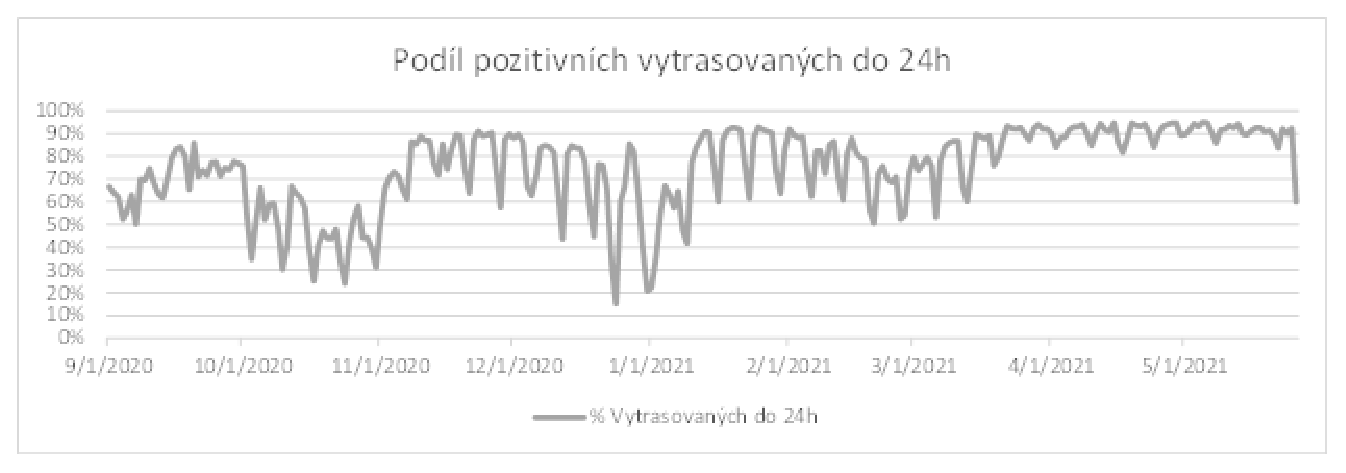
\includegraphics[width=1\textwidth]{./pic/a.eps}
    \caption{Podíl pozitivních případů vytrasovaných do 24 hodin.}
    \label{fig:pozitivni24}
\end{figure}

Celkový přehled podílu pozitivních případů vytrasovaných do 24 hodin v~období od září 2020 do května 2021 je znázorněn na obrázku 2. V~období od 1.~října do 1.~listopadu 2020 se systému trasování dařilo v~průměru obvolat jen 50 \% pozitivních případů do 24 hodin. Od 1.~listopadu do 1.~prosince 2020 to bylo v~průměru 79 \%. V~průběhu prosince 2020 klesla rychlost trasování pozitivních do 24 hodin na průměr 67 \%. V~lednu a únoru 2021 se zvýšila a držela na průměru 73--75 \%. V~březnu 2021 se dostala nad úroveň listopadu 2020 na 83 \% a od dubna 2021 do května 2021 se dokonce drží na průměrné úrovni 90 \%. Systém tedy dosahuje zmiňovaných cílů až od dubna 2021.

Významný souvislý výpadek výkonnosti souvisí s~vánočními svátky. Mezi 18.~prosincem 2020 a 2.~lednem 2021 se podařilo do 24 hodin v~průměrném dni obvolat jen 53 \% pozitivních případů. Výpadek systému trasování tak pravděpodobně přispěl k~prudkému nárůstu nových případů v~lednu 2021 a třetí vlně pandemie covid-19 v~ČR.

Rychlost trasování se zásadním způsobem vylepšila na přelomu roku 2020 a 2021, zejména díky využití profesionálních call center od ledna 2021, včetně veřejné zakázky pro dynamický nákupní systém \cite{tr_hlidac01}.

\begin{figure}[ht]
    \centering
    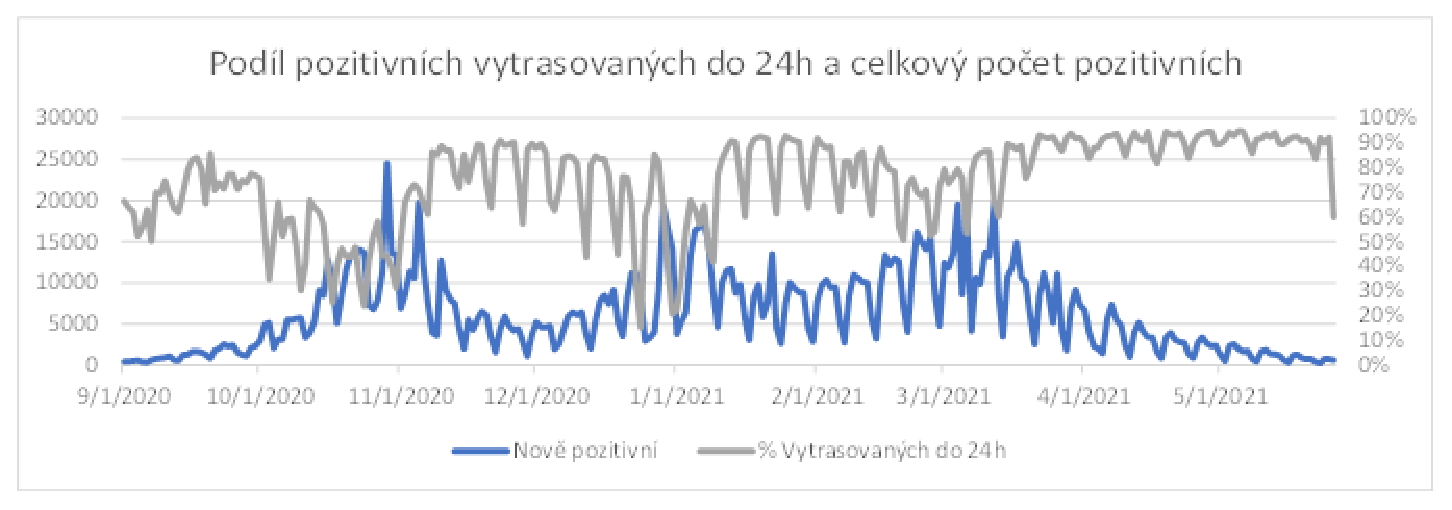
\includegraphics[width=1\textwidth]{./pic/b.eps}
    \caption{Podíl pozitivních případů vytrasovaných do 24 hodin (pravá osa) a celkový počet pozitivních podle registrací v~systému Daktela v~daný den (levá osa).}
    \label{fig:pozitivni24_2}
\end{figure}

Na obr. \ref{fig:pozitivni24_3} srovnáváme vývoj epidemie (denní počty počty nových případů registrovaných v~systému Daktela) a rychlost trasování pozitivních případů (\% do 24 hodin). Z~grafu jasně vyplývá, že trasovací kapacity nebyly od října až do konce roku 2020 dostatečně připravené. Průměrný denní počet případů od 1.~ledna 2021 do 31.~března 2021 (necelých 9 500 případů denně) byl zhruba o~třetinu vyšší než od 1. října do 31. prosince 2020 (necelých 7 200 případů denně). Přesto se při efektivnějším zapojení externích call center v~období od ledna do března 2021 dařilo vytrasovat v~průměrném dni 77 \% pozitivních do 24 hodin, zatímco v~období od října do prosince 2020 to bylo v~průměru jen 65 \% -- při významně vyšším počtu případů.

Zapojení profesionálních call center významně zvýšilo výkon celého systému trasování. Systém byl díky němu na jaře schopen fungovat efektivněji (zhruba~o 20 \%) při významně větším počtu pozitivních případů (o~zhruba 30 \%).

O~to více se nabízí otázka, proč ČR nasadila toto řešení s~pětiměsíčním zpožděním a neměla tyto kapacity připravené v~září 2020. Identické řešení jsme navrhovali jako skupina dobrovolníků v~květnu 2020 \cite{tr_hlidac02} a vláda se k~němu dokonce zavázala svým rozhodnutím z~25.~5. \cite{tr_vlada01}.

\begin{figure}[ht]
    \centering
    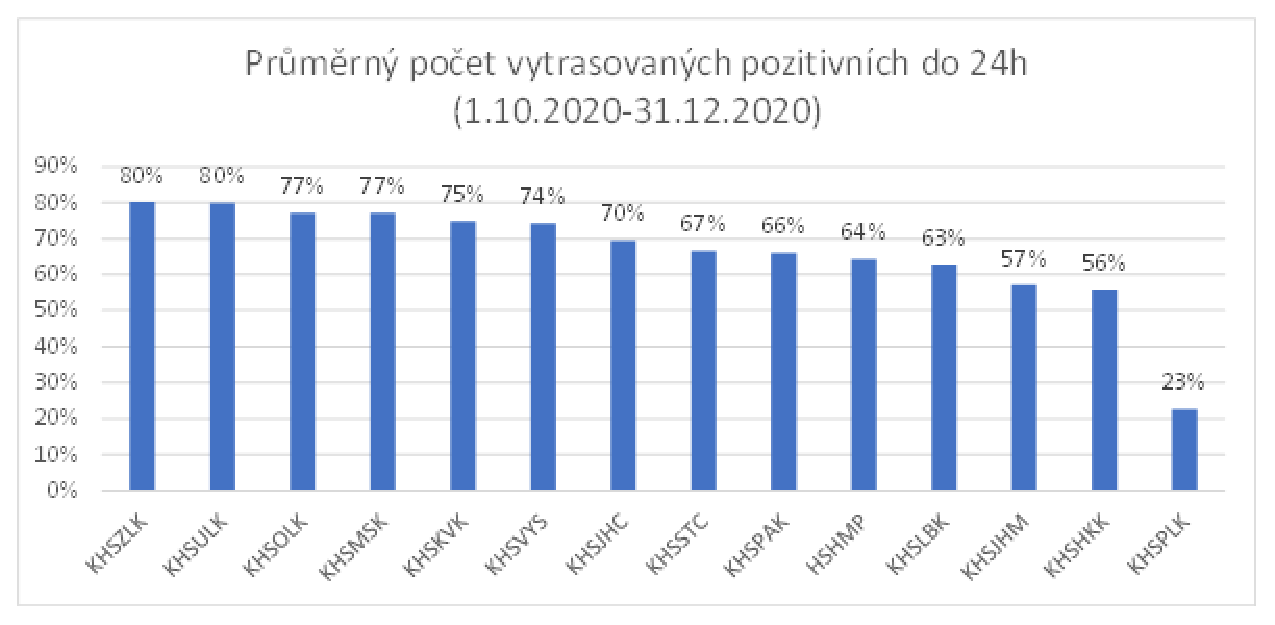
\includegraphics[width=1\textwidth]{./pic/c.eps}
    \caption{Průměrné procento vytrasovaných pozitivních případů do 24 hodin po krajích.}
    \label{fig:pozitivni24_3}
\end{figure}

Výsledky systému se zároveň významně lišily po jednotlivých krajích: zatímco ve Zlínském nebo Ústeckém kraji v~období od října do prosince 2020 v~průměrném dni dokázaly KHS vytrasovat 80 \% pozitivních do 24 hodin, v~Jihomoravském nebo Královéhradeckém kraji to bylo 57 \%, resp. 56 \%. Pracovníci KHS Plzeň však dokázali v~průměrném dni obvolat jen 23 \% pozitivních do 24 hodin.

Regionální rozdílnost výkonnosti jasně ukazuje na největší výše zmíněný deficit systému trasování a to absenci využívání reportingu pro řízení a zlepšování procesů. Násobně nižší výkonnost KHS v~Plzni na podzim 2020 nebyla nikdy veřejně vysvětlena a až do zapojení externích call center nedošlo k~nápravě situace. Na násobné rozdíly její výkonnosti jsme několikrát upozorňovali \cite{tr_bisop03}.

\begin{figure}[ht]
    \centering
    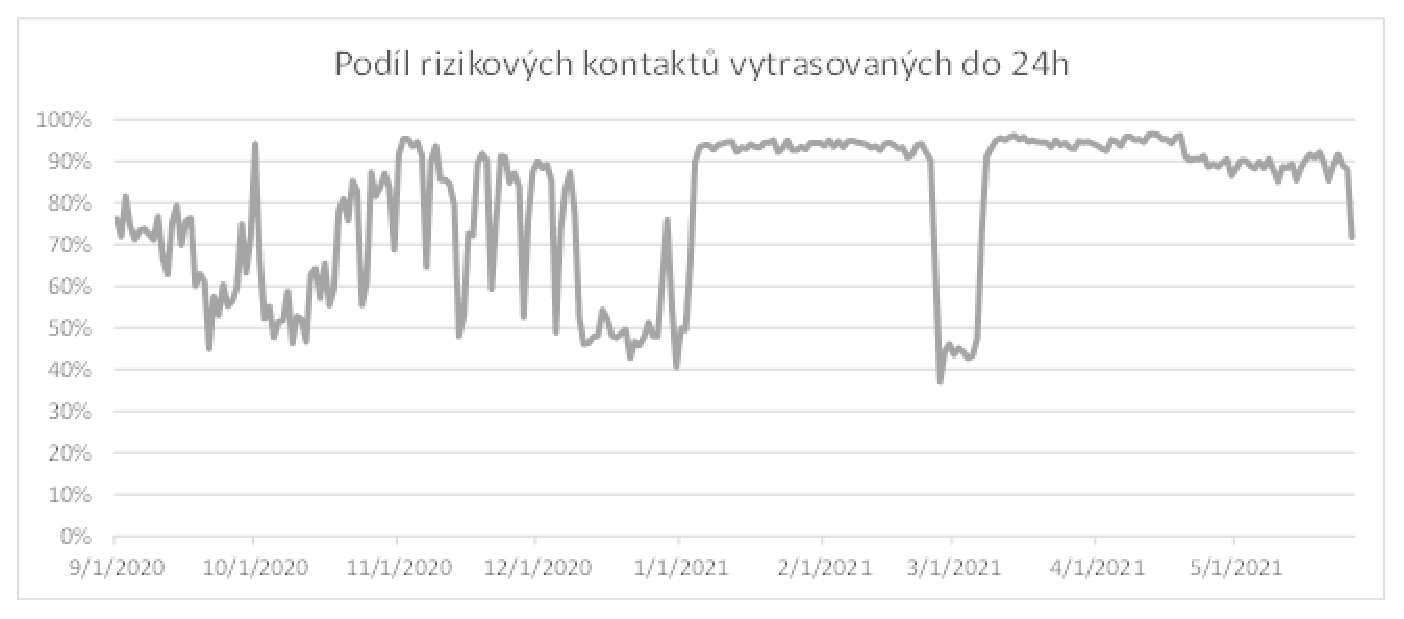
\includegraphics[width=1\textwidth]{./pic/d.eps}
    \caption{Podíl rizikových kontaktů vytrasovaných do 24 hodin, celá ČR}
    \label{fig:rizikove24}
\end{figure}

Rychlost trasování rizikových kontaktů byla v~průměru o~něco vyšší než v~případě trasování pozitivních případů. Od 1. října 2020 do 31. prosince 2020 se v~průměrném dni podařilo vytrasovat 69 \% rizikových kontaktů do 24 hodin od telefonátu s~pozitivním (versus 65 \% v~případě pozitivních kontaktů). Od 1. ledna 2021 je to díky zapojení externích call center stabilně přes 90 \%.

Významný pokles výkonnosti systému nastal mezi 10. 12. 2020 a 2. 1. 2021, kdy se v~průměru podařilo obvolat jen 50 \% rizikových kontaktů do 24 hodin. Tedy podobně jako v~případě rychlosti trasování pozitivních.

Několik dalších zemí též pravidelně zveřejňuje indikátor rychlosti trasování. Je třeba si ale uvědomit, že se metodiky výpočtu mohou v~různých zemích lišit.

\begin{itemize}
\item Australský stát Victoria dosahuje většinou 100\% úspěšnosti trasování jak pozitivních, tak rizikových kontaktů do 24 hodin, ovšem jedná se spíše o~jednotky osob \cite{tr_victoria}.
\item Ve Skotsku se od ledna 2021 hodnoty vytrasovaných pozitivních do 24 hodin pohybují mezi 80 a 95 \%, od října do prosince 2020 týdenní průměry oscilovaly mezi 40 a 85 \% \cite{tr_scotland}.
\item Anglie sleduje počet pozitivních, které se podaří oslovit („reached“) -- za celé reportované období červen 2020 - květen 2021 je průměr 87 \%. Z~těchto osob se pak daří do 24 hodin trasovat 72 \%. Do 24 hodin je poté vytrasováno 92 \% jejich rizikových kontaktů. Hodnoty indikátorů se postupně vylepšují, výše uvedené hodnoty za květen 2021 jsou 91 \%, 82 \%, 98 \% (týden 6.--12. 5. 2021, \cite{tr_gov_uk})
\item Podobné metriky sledují i některé americké státy -- Washington D.C. monitoruje procento případů kontaktovaných do tří dnů, to se od října 2020 do května 2021 pohybuje v~rozmezí převážně 70--80 \% \cite{tr_DC}, Delaware reportuje za období červenec 2020 -- květen 2021 80~\% oslovených („reached“) a z~nich 67 \% vytrasovaných 24 hodin \cite{tr_Delaware}, New Jersey 67 \% vytrasovaných pozitivních do 24 hodin v~týdnu od 16.--22 .5. 2021 \cite{tr_NewJersey}.
\end{itemize}

% \subsection*{Počet identifikovaných rizikových kontaktů}

\paragraph{Počet identifikovaných rizikových kontaktů.} Zatímco počet obvolaných pozitivních případů a identifikovaných kontaktů do 24 h vyjadřuje efektivitu využívání kapacit programu, počet identifikovaných rizikových kontaktů představuje indikátor kvality trasovacího hovoru.

Definice rizikového kontaktu se v~průběhu epidemie měnila -- na začátku pandemie se jednalo o~kontakt ve vzdálenosti 2 metry s~trváním nejméně 15 minut, v září 2020 byla tato definice upravena (kontakt nebyl považován za rizikový pokud jedna z~osob měla zakryté dýchací cesty \cite{tr_MZCR}. K~29. květnu 2021 je rizikový kontakt definován jako kontakt na méně než 2 metry, při kterém alespoň jedna osoba nemá náležitou ochranu dýchacích cest. Časový údaj již není blíže definován. Z~této definice jsou vyjmuty naočkované osoby a osoby, které prodělaly covid-19 v~posledních šesti měsících \cite{tr_covidgov}.

Průměrný počet identifikovaných rizikových kontaktů osciloval od začátku reportingu v~říjnu 2020 na úrovni 0,8--1,3 rizikových kontaktů na jednoho pozitivního. Mezi listopadem 2020 a dubnem 2021 na úrovni 0,8--1,0. Počet identifikovaných rizikových kontaktů začal výrazněji růst na konci dubna 2021 a v~květnu se blížil hodnotě 1,3.

\begin{figure}[ht]
    \centering
    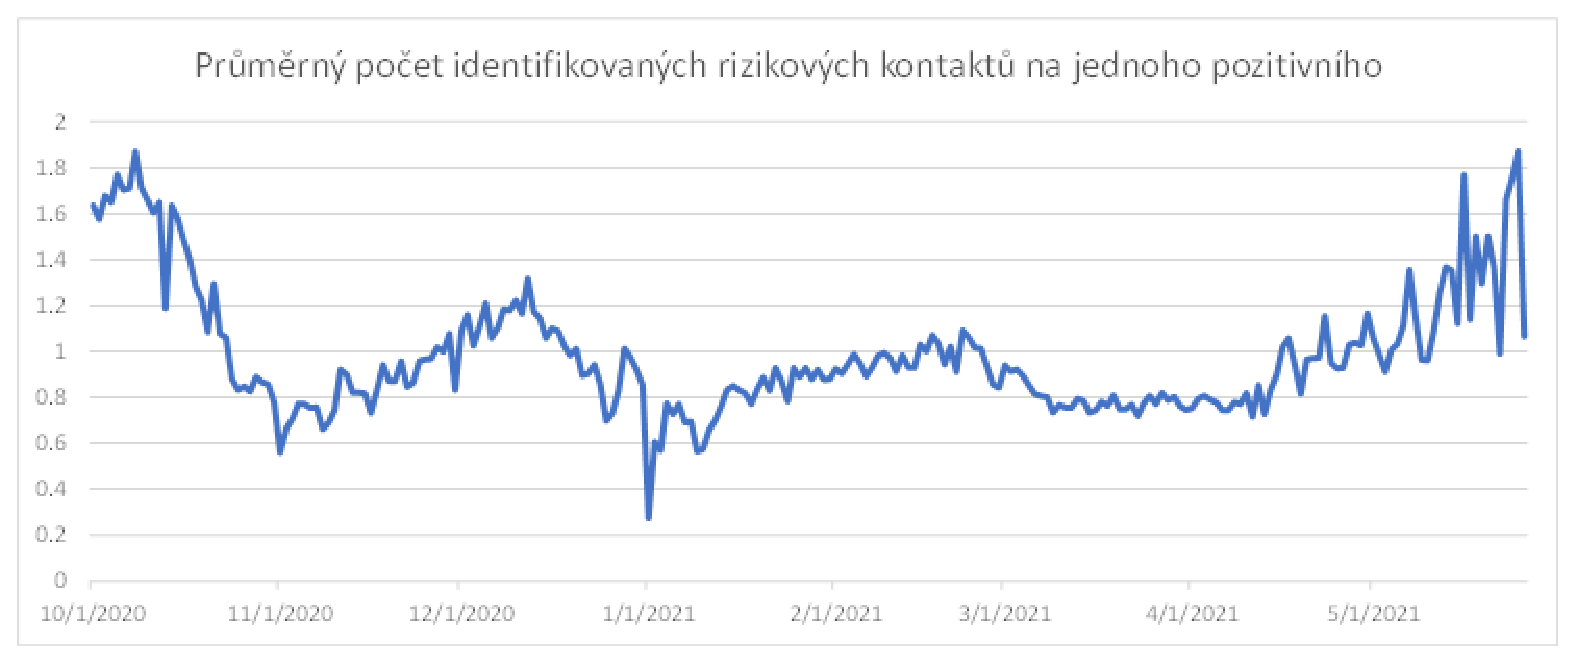
\includegraphics[width=1\textwidth]{./pic/e.eps}
    \caption{Průměrný počet rizikových kontaktů na jednoho pozitivního, celá ČR.}
    \label{fig:rizik1}
\end{figure}

Rozdíly v~počtu identifikovaných rizikových kontaktů mezi kraji jsou ještě vý\-raz\-něj\-ší než pro rychlost trasování. Zatímco za celé období od září 2020 do května 2021 dokázali trasovači ve Zlínském kraji identifikovat v~průměru 1,7 rizikového kontaktu na jednoho pozitivního, v~Jihočeském, Hradeckém a Libereckém kraji to bylo pouze 0,9. Stejně jako v~případě rychlosti vykazuje násobně nižší výsledky Plzeňský kraj s~0,4 identifikovaného rizikového kontaktu na jednoho pozitivního. Na tyto rozdíly jsme upozorňovali na podzim 2020 \cite{tr_bisop04}.

\begin{figure}[ht]
    \centering
    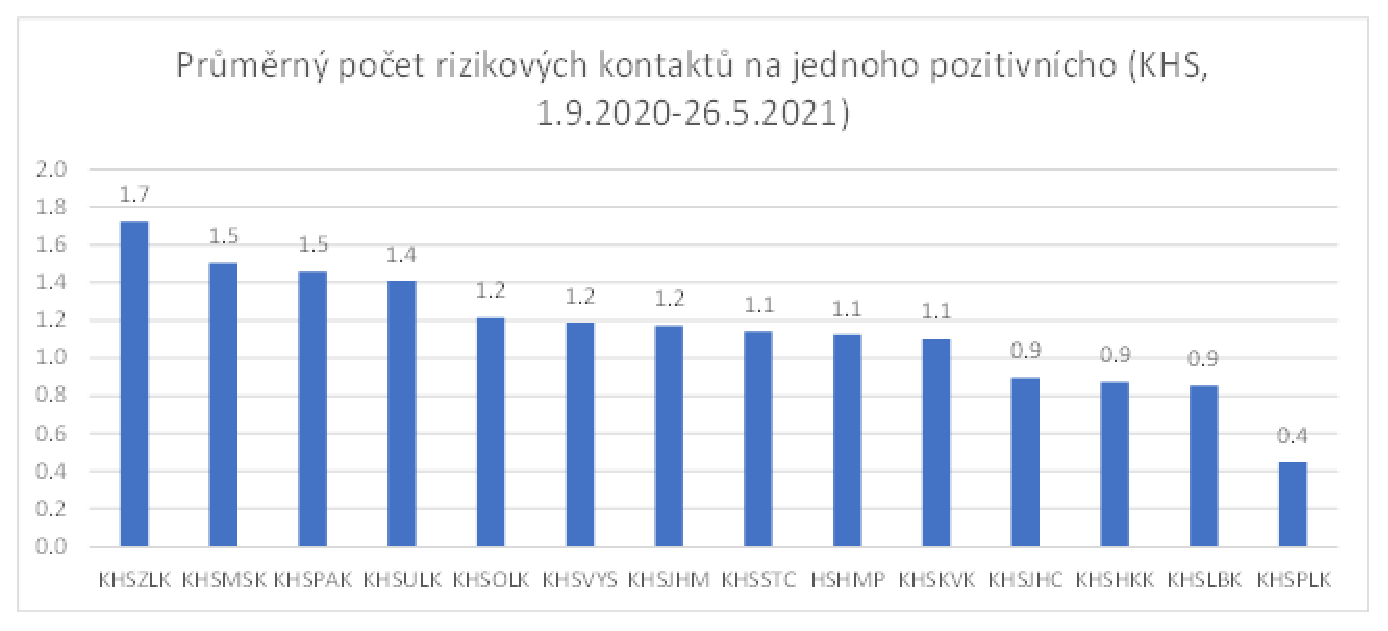
\includegraphics[width=1\textwidth]{./pic/f.eps}
    \caption{Průměrný počet rizikových kontaktů na jednoho pozitivního po krajích.}
    \label{fig:rizik1kraj}
\end{figure}

V~případě identifikovaných rizikových kontaktů chyběly jakékoli indikace cílových hodnot tohoto indikátoru. Systém trasování za celou dobu svého fungování jasně nestanovil, jestli je v~průměru jeden identifikovaný rizikový kontakt adekvátním výstupem trasování nebo jestli je nedostatečný.

Regionální variabilita ukazuje, že významným způsobem záleží na praxi trasování dané hygienické stanice a že potenciál počtu identifikovaných kontaktů pro celou ČR byl přinejmenším o~50 \% vyšší než průměr 1,0 od září 2020 do května 2021. (Viz srovnání 1,5 kontaktu v~Pardubickém a 0,9 v~sousedním a v~mnoha ohledech srovnatelném Královéhradeckém kraji.) Pro dosažení tohoto potenciálu by bylo třeba sledovat, jak se liší praxe trasování ve čtyřech nejlepších krajích od praxe ve zbytku krajích a usilovat o~její implementaci ve zbytku ČR. Nakolik je nám známo k~podobné iniciativě nikdy nedošlo.

Cílová hodnota skutečného počtu rizikových kontaktů však pravděpodobně měla být stanovena výše. Podle sociologických dat šetření \uv{Život během pandemie} \cite{tr_PAQ01} se počet kontaktů respondentů šetření po dobu 15 minut bez ochrany nosu a úst od 12. října 2020 do 11. dubna 2021 pohyboval mezi 4,5--5,5 kontakty. S~ohledem na to, že šetření zjišťuje počet kontaktů v~posledním týdnu a trasování sleduje posledních 48 hodin, by podle šetření cílová hodnota v~tomto období měla být stanovena přibližně na 3 rizikové kontakty na jednoho pozitivního.

Tento cíl odpovídá zkušenostem z~pilotu zavádění Chytré karantény v~Brně na začátku dubna 2020, kdy se v~průměru dařilo identifikovat 4 rizikové kontakty na jeden pozitivní případ.\footnote{Eva Blechová -- archiv autorky.} Podle dat \cite{tr_PAQ01} měli respondenti i tehdy 4,0--4,5 kontaktu delší než 15 minut bez roušky.

Výsledky pilotu chytré karantény a sociologická data PAQ by tak podpořily hypotézu, že počet rizikových kontaktů na pozitivního byl závislý spíše na ochotě občanů spolupracovat se systémem trasování než odrazem skutečného počtu kontaktů. Ne\-dů\-věra v~systém trasování přímo souvisí s~vládní komunikací a s~komunikací systému testování a trasování jako celku. Vláda nepracovala na zlepšení reputace trasování \cite{tr_bisop01} a dopad na trasování určitě měl i celkový pokles důvěry občanů ve zvládání epidemie ze strany vlády (ta klesla z~83 \% v~březnu/dubnu 2020 na 25 \% v~dubnu 2021 \cite{tr_STEM}.Tuto část bylo možné ovlivnit řízením kvality trasovacích rozhovorů, jejich standardizací a využíváním behaviorálních technik zaměřených na vzpomínání (více viz \cite{tr_bisop06}). Nakolik je nám známo, nebylo s~tímto potenciálem nijak systematicky pracováno.

Cílová hodnota systému trasování na úrovni tří kontaktů na jednoho pozitivního v~průběhu plošných omezujících opatření od října 2020 do dubna 2021 by zhruba odpovídala hodnotám dosaženým i v~jiných zemích. Je ovšem potřeba zmínit, že metodologie výpočtu rizikových kontaktů se může podstatně lišit. 
\begin{itemize}
\item Ve Skotsku v~období září 2020 -- květen 2021 osciluje počet RK/pozitivního mezi 3 a 7 \cite{tr_scotland01}.
\item V~Irsku pro osoby, které nahlásily alespoň jeden rizikový kontakt, byl průměr v~květnu 2021~3,5 \cite{tr_irland}. V~roce 2020 se pohyboval mezi 2 a 7 \cite{tr_mcaloon_numbers_2021}.
\item Počet rizikových kontaktů na pozitivního ve Francii se v~roce 2021 pohybuje okolo 2 osob \cite{tr_france}. Na jaře 2020 se v~době přísných omezení blížil číslu 4.
\item Studie provedená v~lednu--březnu 2020 v~Jižní Koreji stanovuje průměrný počet 10,4 \cite{tr_park}.
\item Výsledkům z~ČR jsou nejblíže výsledky ze Spojených států amerických. V~Delaware průměr 2,4 pro pozitivní, kteří jmenovali alespoň jeden kontakt \cite{tr_Delaware}, 1,8 v~Marylandu \cite{tr_maryland01}, ve Washingtonu D.C. je dlouhodobě indikátor mezi 1 -- 2, v~květnu 2021 na hodnotě 1,3 \cite{tr_DC}.
\end{itemize}

V~silách systému trasování samotného bylo přinejmenším zvýšení na 1,5 rizikového kontaktu, tedy na zhruba 50 \% ideálního výkonu, jak vyplývá z~analýzy regionální variability výsledků výše. Určitá část zbylého 1,5 kontaktu byla dána nejen interními rezervami systému trasování, ale i externími podmínkami trasování, především mírou důvěry obyvatel v~systém a jejich spolupráce.

\section*{Diskuse (interpretace)}

Naším cílem bylo celkové vyhodnocení systému trasování za posledních osm měsíců. Pokud je nám známo, jedná se o~jedinou veřejně dostupnou analýzu podobného typu v~ČR. Dospěli jsme ke třem hlavním závěrům:

\begin{enumerate}
\item Ve sledovaném období se rychlost trasování, klíčová pro jeho efektivitu, zá\-sad\-ním způsobem zlepšila. K~tomu došlo zejména díky zavedení jednotného IT sys\-té\-mu a zapojení externích call center. I~při denním počtu případů o~30 \% vyšším se díky zapojení externích call center v~období leden--březen 2021 dařilo vytrasovat 77 \% pozitivních do 24 hodin proti 65 \% v~období říjen--prosinec 2020. Identické řešení jsme navrhovali jako skupina dobrovolníků v~květnu 2020 \cite{tr_hlidac02} a vláda se k~němu dokonce zavázala svým rozhodnutím z~25. května 2020 \cite{tr_vlada01}. O~to nepochopitelnější je fakt, že tento systém nebyl připraven už v~létě 2020. Podzimní druhá vlna covid-19 mohla být významně mírnější.
\item Zveřejňování podrobných denních dat o~trasování od října 2020 je potřeba hodnotit pozitivně, stejně jako výběr hlavních indikátorů (rychlost trasování do 24 hodin, počet rizikových kontaktů/pozitivního). Podstatným nedostatkem systému ale bylo, že vyšší úrovně řízení nevyužívaly tato data k~rozhodování. Jednotlivé indikátory neměly (a dodnes nemají) oficiálně stanovené cílové hodnoty. Představitelé státu je nevyužili k~motivaci občanů ke spolupráci se systémem. Pokud byly jimi veřejně interpretovány, dělo se to často nepřesně a bez identifikace kroků ke zlepšení.

I~přes velké nasazení a kvalitní práci mnoha lidí na nižších úrovních se na nejvyšších úrovních (premiér, ministr zdravotnictví, hlavní hygienička) nepodařilo efektivně systém řídit a zlepšovat. Na příkladu trasování je zjevný deficit ve dvou oblastech. Prvním je absence komplexního pohledu (testování, trasování a „compliance“ jako celku), druhým je absence rozhodování na základě dat (tzv. „evidence-based policy making“). Tyto problémy pravidelně identifikuje stát ve svých strategických dokumentech \cite{tr_MVCR, tr_MZP}, k~významnému posunu ovšem nedochází. Doufáme, že pandemie tyto problémy více obnažila a bude moci být katalyzátorem nutných změn ve fungování státní správy (též kapitola \ref{Nove_vyzvy}).
\item Odhadujeme, že počet rizikových kontaktů/pozitivního mohl mít ambici být přibližně třikrát vyšší -- místo hodnot mezi 0,8 a 1,3 by se měl pohybovat okolo 3. Tento nedostatek ukazuje nedostatky v~komplexním pojímání pandemie. Jestliže rychlost trasování je možné ovlivnit dobrým řízením procesu na nižších úrovních, zvýšení počtu identifikovaných kontaktů vyžaduje komplexní, „nadresortní“ chápání. Bylo by potřeba vnímat souvislosti celého systému „testování, trasování, izolace“ a monitorovat jeho různé komponenty (prodlevy v~celém systému, ochotu občanů se
testovat, hlásit kontakty, dodržovat izolaci/karanténu). V~tomto směru se jako nedostatek ukazuje také izolovaný reporting trasování, oddělený od systému testování a celkového managementu epidemie. Komplexní nahlížení by umožnilo
lépe komunikovat s~občany a motivovat je k~dodržování opatření. Je příznačné, že na datech založený podkladový materiál, který přispěl k~zavedení „izolačky“ \cite{tr_MPSV} v~březnu 2021 nevytvořil státní orgán, nýbrž ho připravil nezávislý expert Daniel Prokop z~PAQ Research \cite{tr_PAQ02}.
\end{enumerate}

Limitem naší analýzy je především omezení na systém trasování (bez komplexnějšího náhledu a propojení s~testováním a „compliance“). Tím bohužel ko\-pí\-ru\-je\-me nedostatky komplexního nahlížení zmíněného výše.

Dalším limitem je neúplnost dat -- ač byly KHS požádány provádět všechny hovory pomocí systému Daktela (tedy telefonovat přes počítač), není jisté, do jaké míry tento pokyn respektovaly. Je možné, že někteří pracovníci KHS pokračovali v~předcovidové praxi, tedy používali vlastní telefon se zápisem do oddělených systémů (papír, excelovská tabulka). Data mohou být tedy zejména v~případě některých krajů neúplná a je složité odhadnout míru této neúplnosti.

Při hodnocení reportingu českého systému trasování jsme využili zahraniční inspirace a benchmarky. Při srovnávání přitom neanalyzujeme do hloubky lokální odlišnosti, jako je například hustota osídlení dané země, míra zasažení země onemocněním covid-19, bohatství, míra důvěry v~instituce apod. Tohoto omezení jsme si vědomi, a srovnání proto využíváme jen jako jedno z~měřítek hodnocení českého systému trasování a jeho reportingu.

Naše analýzy nabízejí několik dalších směrů zkoumání.

\begin{itemize}
\item Prvním je stanovení dopadů nižší účinnosti systému na podzim 2020 ve srov\-ná\-ní s~rokem 2021 na vývoj pandemie covid-19 v~ČR. Nabízí se odhadnout náklady dopadů nižší účinnosti trasování během podzimní vlny pandemie a srovnat je s~náklady na zahrnutí externích call center od léta 2020. Téma neefektivního „šetření“ totiž prostupuje celým řízením pandemie \cite{tr_ProkopN, tr_Zidek}.
\item S~tím souvisí i hlubší analýza procesů, které vedly k~podcenění přípravy na druhou vlnu. Jaké byly hlavní bariéry lidské, či organizační (včetně nastavení incentiv)? Nabízí se kvalitativní výzkum pomocí rozhovorů s~hlavními aktéry, který by tyto mechanismy odkryl. Cílem není najít viníky, ale nastavit lepší mechanismy do budoucna.
\item Dalším krokem by mohla být komplexnější analýza celého systému „test, trace, isolate“ a dopad jeho funkčnosti na epidemii. Například pro data o~prodlevách v~testování existují záznamy v~systémech ISIN a Daktela, i když nejsou veřejné. Nevyužitým zdrojem jsou i nahrávky trasovacích hovorů s~pozitivními a rizikovými kontakty.
\item Přirozeným rozšířením hodnocení účinnosti trasování s~ohledem na počty identifikovaných rizikových kontaktů by bylo stanovení vlivu spolupráce občanů se systémem. Provedena by mohla být prostřednictvím analýzy nahrávek hovorů z~jara a podzimu 2020 (některé kraje začaly nahrávat již v~dubnu 2020).
\end{itemize}

\section*{Poděkování}

Rádi bychom poděkovali Jiřímu Havlíčkovi z~týmu Chytré karantény za spolupráci při interpretaci dat.
